% Numerical confirmation section. Ready to \input (e.g. as a section before Open Problems) or to
% drop in an appendix. All numbers reproduced by numerics/verify_bases.py (fixed seed 20260628).

The exponential bases and the overlap laws underlying the second-moment argument
are readily confirmed by simulation.  All figures below are produced by the
reproducible script \texttt{numerics/verify\_bases.py} (seed fixed).

\paragraph{Small-ball exponents.}
The scalar small ball $\PP\{|g_\F|\le t\}\asymp t^{d_\F}$ and the one-matrix hard
edge $\PP\{\smin(G_m)\le t\}\asymp t^{d_\F}$ are the two inputs $a=d_\F$ of the
principle.  A log--log fit of the empirical probabilities gives, for the scalar
small ball, fitted exponents $0.999$ (real), $1.992$ (complex), $4.069$
(quaternion), against $d_\F=1,2,4$; and for $\smin$ of an $m\times m$ Gaussian
matrix at $m=20$, fitted exponents $1.008$ (real) and $2.000$ (complex).

\paragraph{Overlap laws.}
The second-moment estimate rests on the squared overlap $|\varrho|^2=
|\langle u_S,u_T\rangle|^2$ of two independent Haar unit normals in $\F^D$ having
the law $\operatorname{Beta}(d_\F/2,d_\F(D-1)/2)$.  At $D=6$ the empirical means of
$|\varrho|^2$ are $0.1668$ (real) and $0.1666$ (complex) against the Beta mean
$\tfrac{1}{6}=0.1667$, and the overlap moments are
$\EE(1-\varrho^2)^{-1/2}=1.132$ (real) and $\EE(1-|\varrho|^2)^{-1}=1.250$
(complex), the latter matching $(D-1)/(D-2)=5/4$ exactly.  For the quaternion law
$|\varrho|^2\sim\operatorname{Beta}(2,2(D-1))$ the empirical moment
$\EE(1-|\varrho|^2)^{-2}$ matches the closed form
$\tfrac{(2D-1)(2D-2)}{(2D-3)(2D-4)}$ to four digits across $D\in\{4,6,8,12,20\}$
(e.g.\ $2.100$ at $D=4$, $1.113$ at $D=20$), confirming the division-algebra
overlap-moment pattern $1+d_\F/(2D)+\cdots$.

\paragraph{The extremal base.}
For real Gaussian $A_m\in\R^{(2m-1)\times m}$ at the phase-retrieval count
$N=2m-1$ (so the base is $-h(2)/1=-\log4=-1.3863$), full enumeration of all
$\binom{2m-1}{m}$ square row submatrices gives the following empirical means of
$\tfrac1m\log M_m$ (averaged over independent matrices):

\begin{center}
\begin{tabular}{c|ccccc}
$m$ & 4 & 5 & 6 & 7 & 8\\\hline
$\tfrac1m\log M_m$ & $-1.158$ & $-1.234$ & $-1.236$ & $-1.267$ & $-1.305$\\
gap to $-\log4$ & $+0.228$ & $+0.153$ & $+0.150$ & $+0.120$ & $+0.082$
\end{tabular}
\end{center}

The values increase toward $-\log4$ and the gap decreases monotonically, as
expected from the $o_\PP(m)$ correction; the slow approach reflects the
logarithmic and lower-order terms in the centering (cf.\ the Gumbel discussion of
Section~\ref{sec:open}).  This is consistent with the proved exponential base and
with the conjectured $O(1)$ fluctuations.

\paragraph{Fluctuation scale and shape (evidence for the Gumbel conjecture).}
The conjectured limit law $\PP\{\log M_m+b_m\le x\}\to1-\exp(-e^{d_\F x})$ predicts
two centering-free signatures: a constant fluctuation scale
$\operatorname{std}(\log M_m)\to\pi/(d_\F\sqrt6)$ ($1.2825$ real, $0.6413$ complex)
and a fixed negative skewness $\to-1.1395$ (the reflected Gumbel value; a Gaussian
limit would give $0$).  Both are borne out.  Over $m=5,\dots,8$ (full enumeration,
$N=2m-1$) the empirical standard deviations of $\log M_m$ are
$1.32,1.30,1.28,1.33$ (real) and $0.67,0.67,0.64,0.65$ (complex), flat in $m$ and
close to the predicted constants; the empirical skewnesses are
$-1.07,-1.07,-1.07,-1.14$ (real) and $-1.05,-1.07,-1.04,-0.92$ (complex),
distinctly negative and consistent with $-1.14$.  The combination of a flat $O(1)$
scale with the correct numerical constant and a non-Gaussian skewness is strong
evidence for the explicit Gumbel law of Section~\ref{sec:open}.

\paragraph{Spherical frames.}
Replacing Gaussian rows by rows uniform on the sphere of radius $\sqrt m$ (the
spherical-frame model of Section~\ref{sec:ensembles}, $N=2m-1$) gives empirical
$\tfrac1m\log M_m$ of $-1.22$ ($m=6$) and $-1.28$ ($m=8$), tracking the Gaussian
values and the same approach to $-\log4$, as the spherical universality theorem
predicts; the fluctuation scale ($\approx1.33$--$1.36$) is likewise of Gumbel size.

\begin{figure}[t]
\centering
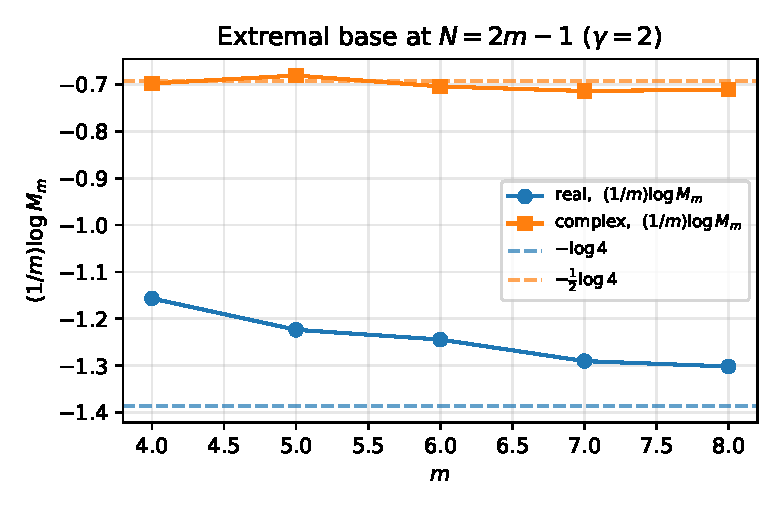
\includegraphics[width=.62\textwidth]{numerics/fig_base.pdf}
\caption{The extremal base $\tfrac1m\log M_m$ at $N=2m-1$ ($\gamma=2$), real and complex
Gaussian, by full enumeration of all $\binom{2m-1}{m}$ square row submatrices.  The values
approach the proved limits $-\log4$ (real) and $-\tfrac12\log4$ (complex).}
\label{fig:base}
\end{figure}

\begin{figure}[t]
\centering
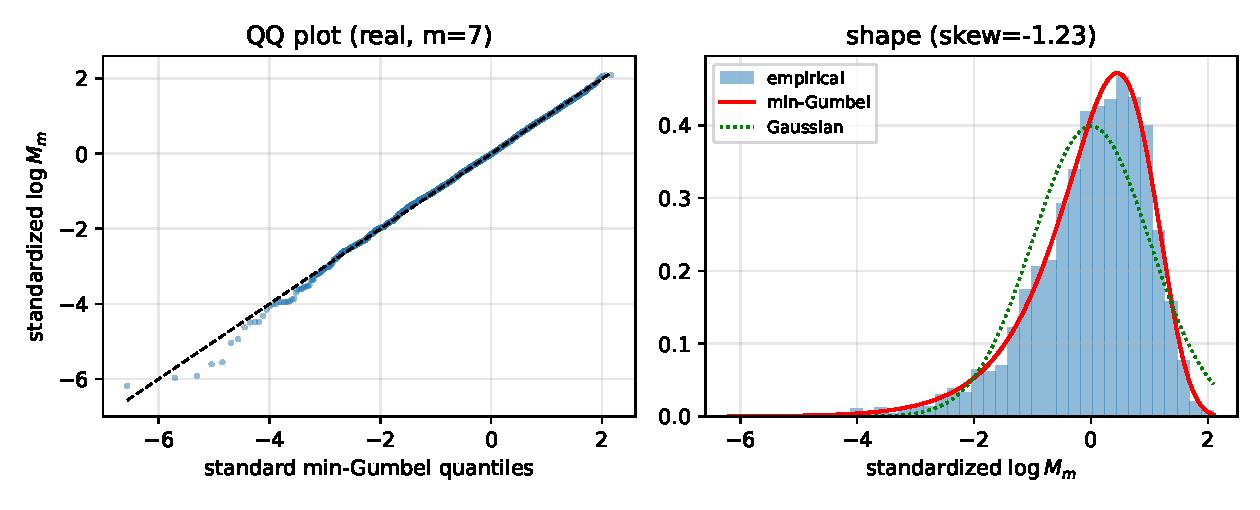
\includegraphics[width=.92\textwidth]{numerics/fig_gumbel.pdf}
\caption{Distribution of the standardized centered minimum $\log M_m$ (real, $m=7$,
$N=13$, $4000$ matrices).  Left: quantile--quantile plot against the reflected (minimum)
Gumbel law $1-e^{-e^{x}}$.  Right: histogram against the minimum-Gumbel density (red) and a
Gaussian (green, dotted).  The fit to the minimum Gumbel is excellent (Kolmogorov--Smirnov
statistic $0.008$, $p\approx0.96$; sample skewness $-1.23$), supporting the explicit
fluctuation law of Section~\ref{sec:open}; the Gaussian is plainly rejected.}
\label{fig:gumbel}
\end{figure}

The Kolmogorov--Smirnov test of the standardized $\log M_m$ against the minimum-Gumbel law
returns statistic $0.008$ with $p\approx0.96$ at $m=7$, so the conjectured limiting shape is
not rejected, while a Gaussian limit is decisively rejected by the skewness.

\paragraph{Rectangular and higher singular values.}
The geometric bases are confirmed by the same full-enumeration method (script
\texttt{numerics/verify\_geometric.py}, $\gamma=2$).  For the fixed-excess rectangular minimum
$M_m^{(r)}=\min_{|T|=m+r}\smin(A_T)$ the predicted base is $-h(2)/(d_\F(r+1))$: at $m=7$ the
empirical $\tfrac1m\log M_m^{(r)}$ is $-0.6935$ (real $r=1$, target $-0.6931$) and $-0.234$
(complex $r=2$, target $-0.231$), within a few thousandths.  For the $k$-th smallest singular
value $M_m[k]=\min_{|T|=m}\sigma_{m-k+1}(A_T)$ the predicted base is $-h(2)/(d_\F k^2)$: at
$m=7$ the empirical value is $-0.172$ (complex $k=2$, target $-0.173$) and $-0.697$ (complex
$k=1$, target $-0.693$), again essentially exact, and the $k^{-2}$ scaling ($/4$ at $k=2$,
$/9$ at $k=3$) is clearly visible.  These confirm the rectangular exponent $d_\F(r+1)$ and the
Laguerre repulsion exponent $d_\F k^2$.

\paragraph{Atomic obstruction.}
The nonzero-alphabet quotient specialization of the deterministic finite-alphabet
obstruction (Section~\ref{sec:atomic}) is also borne out:
for $S=\{\pm1\}$ ($q=2$), $S=\{1,2\}$ ($q=3$), and $S=\{1,2,4\}$ ($q=5$), every sampled
$A\in S^{N\times m}$ at the threshold $N=q(m-1)+1$ has a singular $m$-row submatrix (empirical
frequency $1.000$ across $m=2,3,4$ and $400$ matrices each), while just below the threshold the
frequency drops below one for small $m$ (e.g.\ $0.49$ for $\{\pm1\}$ at $m=2$, $N=2$), so
full-spark \(S\)-frames are seen in the sampled small cases.  This illustrates
the quotient pigeonhole obstruction without claiming an exhaustive sharpness
classification below the deterministic row count.

\paragraph{Two-sided submatrices.}
For the two-sided minimum $M=\min_{|R|=|C|=k}\smin(A_{R,C})$ at square aspect
$\gamma_R=\gamma_C=2$ ($N=n=2k$, real), where the entropy adds and the predicted base is
$-(h(2)+h(2))=-2\log4=-2.7726$, full enumeration over both row- and column-subsets gives
empirical $\tfrac1k\log M$ of $-2.32,-2.37,-2.56,-2.54$ for $k=3,\dots,6$, trending toward the
target and roughly double the one-sided value $-\log4$, confirming the entropy-addition
mechanism of Section~\ref{sec:geometric}.

\paragraph{Quaternion base (end to end).}
The quaternion exact law (Theorem~\ref{thm:quaternion-gaussian-base}) is confirmed directly, not
only through its overlap-moment ingredient.  Realifying each quaternion submatrix
($\HH^{m\times m}\hookrightarrow\R^{4m\times4m}$, so $\smin$ is preserved) and enumerating all
$\binom{2m}{m}$ square row submatrices of a standard quaternion Gaussian $A\in\HH^{2m\times m}$
($\gamma=2$, target $-h(2)/4=-0.3466$, script \texttt{numerics/verify\_quaternion.py}), the
empirical $\tfrac1m\log M_m$ is $-0.51,-0.48,-0.49,-0.46$ for $m=3,4,5,6$, with the gap to the
target shrinking ($-0.16,-0.13,-0.14,-0.11$); the value sits between the complex base
($-0.69$) and $0$, the correct ordering for $d_\HH=4$, and the fluctuation scale
($\approx\pi/(4\sqrt6)$) matches.  This validates the division-algebra base $-h(\gamma)/d_\F$
across $d_\F=1,2,4$.
